\section{Classical Runge-Kutta method}

\subsection{Description of Runge-Kutta}
As all other numerical solvers we have seen, Runge-Kutta discretizes the continous ODE by iteratively computing $x_{n+1}$ from $x_n$, i.e. using a finite-difference approximation. But whereas the previous methods take one long step from $x_n$ to $x_{n+1}$, Runge-Kutta is based on first taking multiple in-between steps $X_j$ for $j=1..s$ where $s$ is the number of stages. The computation $x_{n+1}$ is then computed as an weighted average of the stages. The higher number of stages, the higher is the order of the method and therefore also higher the accuracy. For error estimation instead of using step doubling, a higher order method is typically used ($\hat{x}_{n+1}$). The error is the estimated as $e_{n+1}=x_{n+1}-\hat{x}_{n+1}$. All in all the equations are denoted \cite{JrgensenRunge-KuttaEquations}:\\
\underline{Stages}

\begin{equation}
\begin{aligned}
&T_{i}=t_{n}+c_{i} \Delta t_n \quad i=1,2, \ldots, s\\
&X_{i}=x_{n}+\Delta t_n \sum_{j=1}^{s} a_{i j} f\left(T_{j}, X_{j}\right) \quad i=1,2, \ldots, s
\end{aligned}
\end{equation}

Where the full \underline{next step} from $x_n$ to $x_{n+1}$ is calculated by

\begin{equation}
\begin{aligned}
&t_{n+1}=t_{n}+\Delta t_n \\
&x_{n+1}=x_{n}+\Delta t_n \sum_{j=1}^{s} b_{j} f\left(T_{j}, X_{j}\right) \\
&\hat{x}_{n+1}=x_{n}+\Delta t_n \sum_{j=1}^{s} \hat{b}_{j} f\left(T_{j}, X_{j}\right) \\
&e_{n+1}=x_{n+1}-\hat{x}_{n+1}=\Delta t_n \sum_{j=1}^{s} d_{j} f\left(T_{j}, X_{j}\right) \quad d_{j}=b_{j}-\hat{b}_{j}
\end{aligned}
\end{equation}

The Explict and Implicit Euler methods are particular cases of the Runge-Kutta with s=1.

\\\

\textbf{Classical Runge-Kutta}\\
One intuitive idea is to let the stages only depend on previous $X_j$'s leading to Explicit Runge-Kutta methods. The Classical Runge-Kutta is such a method. Additionally, it is a 4 stage method where the different coefficients is chosen as summarized by this Butcher Tableau \cite{JrgensenRunge-KuttaEquations}

$$
\begin{array}{c|cccc}
0 & & & & \\
\frac{1}{2} & \frac{1}{2} & & & \\
\frac{1}{2} & 0 & \frac{1}{2} & & \\
1 & 0 & 0 & 1 & \\
\hline \mathrm{X} & \frac{1}{6} & \frac{1}{3} & \frac{1}{3} & \frac{1}{6}
\end{array}
$$

Which means that $x_{n+1}$ is iteratively calculated by

\begin{equation*}
\begin{array}{ll}
T_{1}=t_{n} & X_{1}=x_{n} \\
T_{2}=t_{n}+\frac{1}{2} \Delta t_n & X_{2}=x_{n}+\Delta t_n \frac{1}{2} f\left(T_{1}, X_{1}\right) \\
T_{3}=t_{n}+\frac{1}{2} \Delta t_n & X_{3}=x_{n}+\Delta t_n \frac{1}{2} f\left(T_{2}, X_{2}\right) \\
T_{4}=t_{n}+\Delta t_n & X_{4}=x_{n}+\Delta t_n f\left(T_{3}, X_{3}\right)
\end{array}
\end{equation*}

\begin{equation}
\begin{aligned}
&t_{n+1}=t_{n}+\Delta t_n \\
&x_{n+1}=x_{n}+\Delta t_n\left(\frac{1}{6} f\left(T_{1}, X_{1}\right)+\frac{1}{3} f\left(T_{2}, X_{2}\right)+\frac{1}{3} f\left(T_{3}, X_{3}\right)+\frac{1}{6} f\left(T_{4}, X_{4}\right)\right)
\end{aligned}
\end{equation}

The classical Runge-Kutta has no embedded method for error estimation.

\subsection{MATLAB implementation fixed step size}
The above mentioned classical Runge-Kutta method is implemented in MATLAB with a fixed step size $\Delta t_n = h$. For easability, the Butcher Tableau is implemented separately for exporting the parameters:

\begin{adjustwidth*}{0cm}{-0.4cm}
\begin{lstlisting}[frame=single, language=Matlab,caption=Classical Runge-Kutta Parameters, label=ERKpars]
function solver = ERKSolverErrorEstimationParameters(method)
% Parameter for specific ERK method
o = nan;
switch upper(method)
    case 'RK44' % Classical Runge-Kutta
        s = 4;

        A = zeros(s,s);
        A(2,1) = 1/2;
        A(3,2) = 1/2;
        A(4,3) = 1;

        b = [1/6; 1/3; 1/3; 1/6];
        c = [0; 1/2; 1/2; 1];
        d = [0; 0; 0; 0]; % Not Aplicable

    otherwise
       error('Method not defined') 
end

solver.AT = A';
solver.b  = b;
solver.c  = c;
solver.d  = d;
solver.o = o;
solver.stages = s;
\end{lstlisting}
\end{adjustwidth*}

The implementation in listing \ref{ERK} is an implementation of the more general family of Explicit Runge-Kutta methods. By exporting the parameters using listing \ref{ERKpars} one arrives as the classical Runge-Kutta.

\begin{adjustwidth*}{0cm}{-0.4cm}
\begin{lstlisting}[frame=single, language=Matlab,caption=Explicit Runge-Kutta, label=ERK]
function [Tout,Xout,Eout] = ...
        ERKSolverErrorEstimation(fun,tspan,x0,h,solver,varargin)
% ERKSOLVERERRORESTIMATION  Fixed step size ERK solver with error est.
%
%                           Solves ODE systems in the form dx/dt = f(t,x)
%                           with x(t0) = x0. 
%
% Syntax:
% [Tout,Xout,Eout]=ERKSolverErrorEstimation(fun,tspan,x0,h,solver,varargin)

% Solver Parameters
s  = solver.stages;     % Number of stages in ERK method
AT = solver.AT;         % Transpose of A-matrix in Butcher tableau
b  = solver.b;          % b-vector in Butcher tableau
c  = solver.c;          % c-vector in Butcher tableau
d  = solver.d;
%o  = solver.o;          % Order

% Parameters related to constant step size
hAT = h*AT;
hb  = h*b;
hc  = h*c;
hd  = h*d;

% Size parameters
x  = x0;                % Initial state
t  = tspan(1);          % Initial time
tf = tspan(end);        % Final time
N = int64( (tf-t)/h );  % Number of steps
nx = length(x0);        % System size (dim(x))

% Allocate memory
T  = zeros(1,s);        % Stage T
X  = zeros(nx,s);       % Stage X
F  = zeros(nx,s);       % Stage F

Tout = zeros(N+1,1);    % Time for output
Xout = zeros(N+1,nx);   % States for output
Eout = zeros(N+1,nx);   % Errors for output

% Algorithm starts here
Tout(1) = t;        
Xout(1,:) = x';
for n=1:N
    % Stage 1
    T(1)   = t;
    X(:,1) = x;
    F(:,1) = fun(T(1),X(:,1),varargin{:});
    
    % Stage 2,3,...,s
    T(2:s) = t + hc(2:s);
    for i=2:s
        X(:,i) = x + F(:,1:i-1)*hAT(1:i-1,i);
        F(:,i) = feval(fun,T(i),X(:,i),varargin{:});
    end
    
    % Next step
    t = t + h;
    x = x + F*hb;
    e = F*hd;
    
    % Save output
    Tout(n+1) = t;
    Xout(n+1,:) = x';
    Eout(n+1,:) = e';
end
\end{lstlisting}
\end{adjustwidth*}




\subsection{MATLAB implementation adaptive step size}
Similarly to listing \ref{ERK}, the below implementation is the more general family of Adaptive Explicit Runge-Kutta methods. By extracting the parameters using listing \ref{ERKpars} one arrives as the classical Runge-Kutta. The error estimation is based on step doubling, iteratively decreasing the step size until the error (as estimated by taking the two half steps) is below specified tolerances. The step doubling procedure is described in full detail in Section \ref{sec:stepdoubling}.

\begin{adjustwidth*}{0cm}{-0.4cm}
\begin{lstlisting}[frame=single, language=Matlab,caption=Adaptive Explicit Runge-Kutta, label=ERK]
function [Tout,Xout,Eout] = ...
        AdaptiveERKSolverErrorEstimation(fun,tspan,x0,h,solver, ...
        abstol, reltol, varargin)
% Epsilon tolerance
epstol=0.8;

% Solver Parameters
s  = solver.stages;     % Number of stages in ERK method
AT = solver.AT;         % Transpose of A-matrix in Butcher tableau
b  = solver.b;          % b-vector in Butcher tableau
c  = solver.c;          % c-vector in Butcher tableau
d  = solver.d;
kpow  = solver.o+1;     % kpow = order + 1

h = h; % Initial step size

% Size parameters
x  = x0;                % Initial state
t  = tspan(1);          % Initial time
tf = tspan(end);        % Final time
nx = length(x0);        % System size (dim(x))

% Allocate memory
T  = zeros(1,s);        % Stage T
X  = zeros(nx,s);       % Stage X
F  = zeros(nx,s);       % Stage F

% More init
Tout = t;        
Xout = x';
Eout = 0;

% Algorithm starts here
while t < tf
    if (t+h > tf) % Don't go too far
        h = tf-t;
    end

    AcceptStep = false;
    while ~AcceptStep
        %%% Runge-Kutta
        % Stage 1
        T(1)   = t;
        X(:,1) = x;
        F(:,1) = fun(T(1),X(:,1),varargin{:});
        
        % Stage 2,3,...,s
        T(2:s) = t + h*c(2:s);
        for i=2:s
            X(:,i) = x + F(:,1:i-1)*h*AT(1:i-1,i);
            F(:,i) = feval(fun,T(i),X(:,i),varargin{:});
        end

        % Estimate of apprixmation error
        e = F*h*d;

        % Controlling step size h relative to error
        r = max(abs(e) ./ max(abstol, abs(x + F*h*b) .*reltol));
        h = (epstol/r)^(1/kpow) * h;

        AcceptStep = (r<=1.0);
        if AcceptStep
            t = t+h;
            x = x + F*h*b;
        end
    end
    % Save output when AcceptStep == true
    Tout = [Tout; t];
    Xout = [Xout; x'];
    Eout = [Eout; e];
end
\end{lstlisting}
\end{adjustwidth*}

\subsection{Van der Pol}

\subsubsection*{Fixed step size}
For ...

\begin{figure}[H]
    \centering
    \includegraphics[width=\textwidth]{plots/}
    \caption{Solution of the state independent diffusion Van der Pol SDE with varying $\sigma$.}
    \label{fig:4b}
\end{figure}

\subsubsection*{Adaptive step size}

\begin{figure}[H]
    \centering
    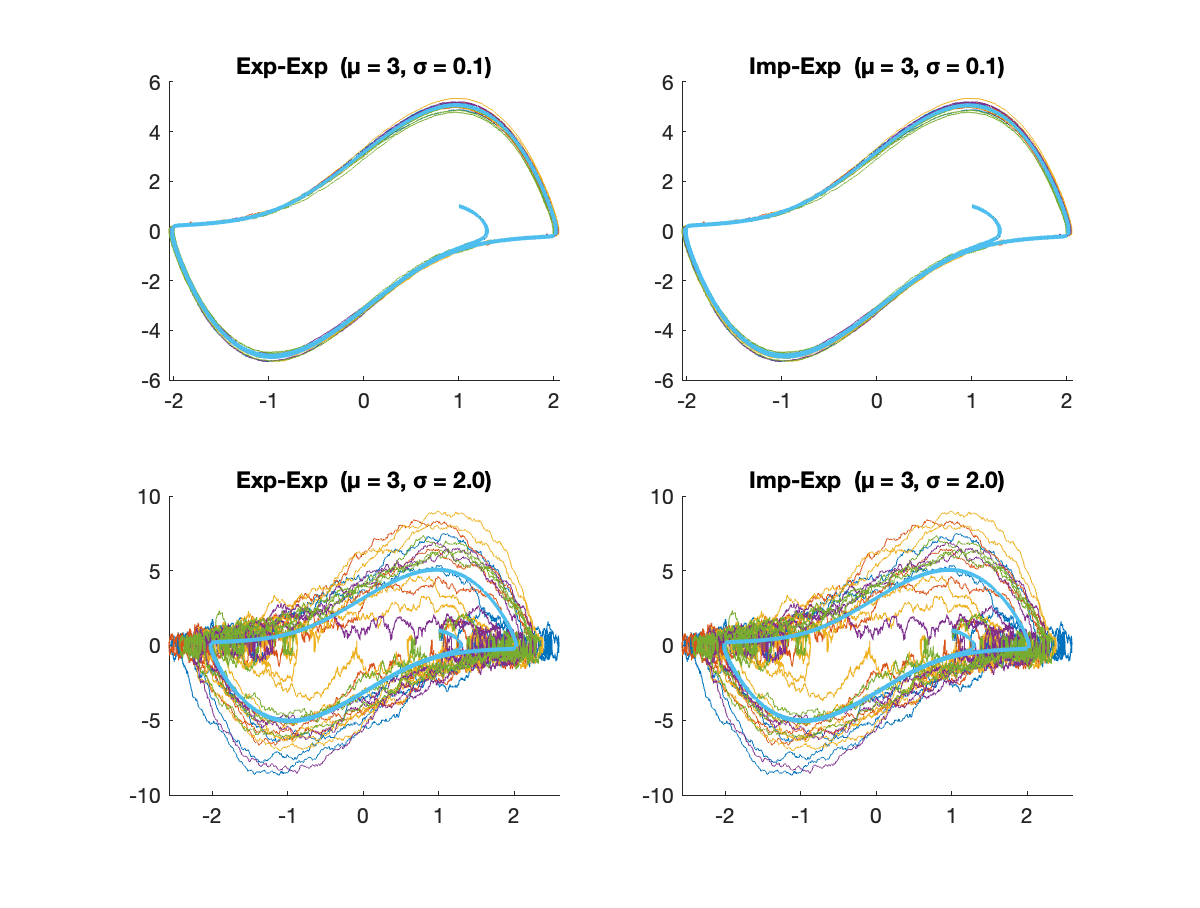
\includegraphics[width=\textwidth]{plots/4b.eps}
    \caption{Solution of the state independent diffusion Van der Pol SDE with varying $\sigma$.}
    \label{fig:4b}
\end{figure}

\begin{figure}[H]
    \centering
    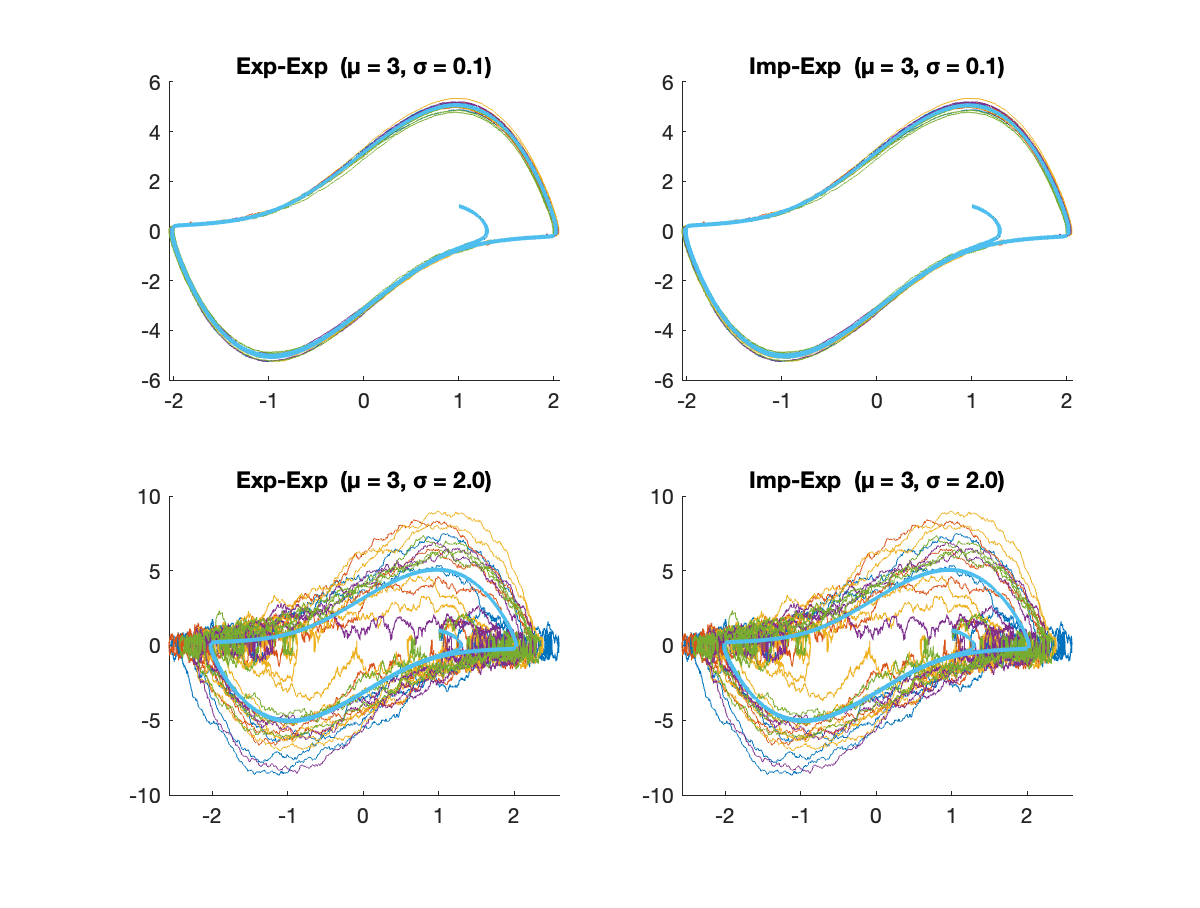
\includegraphics[width=\textwidth]{plots/4b.eps}
    \caption{Solution of the state independent diffusion Van der Pol SDE with varying $\sigma$.}
    \label{fig:4b}
\end{figure}




\subsection{Discussion of interface}